  A torre de sustentação da turbina tem como função suportar todo o peso do rotor e da nacele e erguer este conjunto a uma altura onde as pás possam girar com segurança e distantes do solo. A altura da torre tem uma relação direta com a capacidade de produção de energia, sendo que quanto mais alto a torre for, maior será essa produção devido ao maior fluxo de vento. Com os ventos constantes, o que determinará a quantidade de energia a ser gerada é o diâmetro do rotor. O diâmetro do rotor da turbina tratada neste projeto é de 18,5 m, possuindo um torque médio em seu eixo de   4775, 5 N.m e com a necessidade de gerar 50 kW. A seguir uma breve relação entre o diâmetro do motor e a geração máxima de energia capaz de ser produzida por uma turbina eólica tradicional. \footnotemark
  \footnotetext{<http://www.fiec.org.br/artigos/energia/energia\_eolica.htm>. Acesso em 26 maio de 2015.}
  
  \begin{figure}[!h]
    \centering
    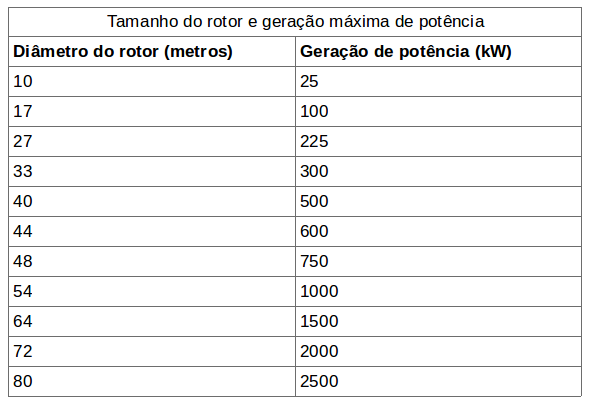
\includegraphics[scale = 0.5]{editaveis/figuras/tamanho_rotor}
    \label{tamanho_rotor}
    \caption[Tamanho do rotor e geração máxima de potência]{Tamanho do rotor e geração máxima de potência. \footnotemark}
   \end{figure}
   \FloatBarrier
   \footnotetext{Fonte: Associação Dinamarquesa da Indústria Eólica, Associação Americana de Energia Eólica.}
   
   Existem três tipos de torre utilizadas para a afinidade buscada: a tubular em aço, a tubular em concreto e a treliçada e quanto ao porte: pequeno, intermediário e grande porte. A turbina do projeto foi enquadrada como porte intermediário (10 - 250kW).  Devido ao aumento do peso dos componentes suportados pela nacele e das próprias pás ao longo dos anos, tem-se usado atualmente as torres tubulares de metais ou de concreto para assegurar a sustentação e suportar tensões provocadas por altitudes cada vez mais altas \footnotemark. Por este motivo e pela elevada preferência pelo mercado nesse tipo de torre, foi escolhido a torre tubular.
   \footnotetext{Disponível em: <http://www.cresesb.cepel.br/download/tutorial/tutorial\_eolica\_2008\_e-book.pdf>. Acesso em: 26 mai. 2015.}
   
   As torres cônicas tubulares podem ser compostos por aço, material relativamente barato e de montagem rápida podendo ser realizada no próprio lugar de instalação; Betão, que pode ser tanto construída no local como pré-moldado, porém é menos flexível que as torres de aço, ou podem ser híbridas, onde sua base é construída de concreto  e seu corpo principal de aço (As torres são frequentemente acoplada com parafusos às concretas bases sobre as quais repousam). \footnotemark
   \footnotetext{Fonte: Energias Renováveis: Energia Eólica 26/06/2014 Por : Luís Timóteo 3.}
   
   Depois de semanas de pesquisas, cruze de dados e comparações entre diversos modelos de torre, a equipe da frente de mecânica optou por utilizar uma torre de aço Q415 que passa por um processo de galvanização quente e pintado com spray, dando a capacidade de proteger a torre contra corrosão e ferrugem. \footnotemark
   \footnotetext{Disponível em: <http://www.chinahummer.cn/index.php/index/content/45>. Acesso em: 19 mai. 2015.}
   
   Partindo do princípio que a velocidade do vento necessária para a produção de energia desejada é a mínima do local de instalação das turbinas, definimos a altura como uma distância segura do solo apenas, tendo em vista que não precisamos colocar o rotor a uma determina altitude para que alcance uma determinada velocidade do vento. Desta forma, escolhemos uma torre com as seguintes especificações: 
   
   \begin{figure}[!h]
    \centering
    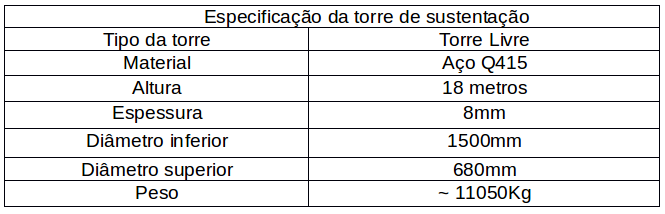
\includegraphics[scale = 0.5]{editaveis/figuras/torre_spec}
    \label{torre_spec}
    \caption[Especificação da torre de sustentação]{Especificação da torre de sustentação. \footnotemark}
   \end{figure}
   \FloatBarrier
   \footnotetext{Disponível em :< http://1047121.en.makepolo.com/products/50KW-Wind-Turbine-Generator-p41716180.html>. Acesso em 20 mai. 2015.}
   
   Quanto ao material utilizado nessa torre, trata-se de um Aço Inox 415. O aço inoxidável pertence à classe Martensítica e possui uma adição de elementos em sua composição química que aumenta a resistência à corrosão em relação aos martensíticos tradicionais. Comparado com os aços 410 e 420, o aço 415 contém uma quantidade menor de carbono, o que confere um diferencial para esta liga. Esta liga passa por um processo de têmpera para  que suas propriedades mecânicas e de dureza se elevem, posteriormente passando também por um processo de revenimento para aliviar as tensões internas do material provocadas pela têmpera. Sua aplicação é importante em ambientes onde o material está exposto a atrito, corrosão e abrasão, devido a estes fatores, a aplicação desta liga na construção de torres de sustentação para turbinas eólicas são constantes.. Devido a estes fatores, a aplicação desta liga na construção de torres de sustentação para turbinas eólicas são constantes. A composição química e as propriedades mecânicas e físicas, estão representados em forma de tabela à seguir [6]:\footnotemark
   \footnotetext{Disponível em:< http://www.megaligas.com.br/produtos\_aco\_inox\_S41500.asp>. Acesso em: 20 mai. 2015.}
     \begin{figure}[!h]
    \centering
    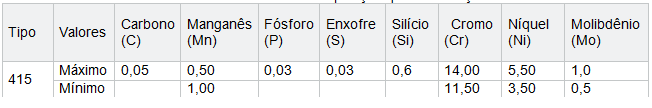
\includegraphics[scale = 1]{editaveis/figuras/composicaco_quimica_415}
    \label{composicao_415}
    \caption[Tabela da composição química do aço 415]{Tabela da composição química do aço 415}
   \end{figure}
   \FloatBarrier
   
    \begin{figure}[!h]
    \centering
    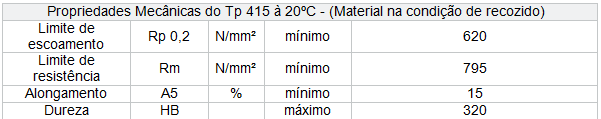
\includegraphics[scale = 1]{editaveis/figuras/propriedade_mecanica_415}
    \label{prop_mec415}
    \caption[Propriedades Mecânicas do Tp 415]{Propriedades Mecânicas do Tp 415}
   \end{figure}
   \FloatBarrier
   
   \begin{figure}[!h]
    \centering
    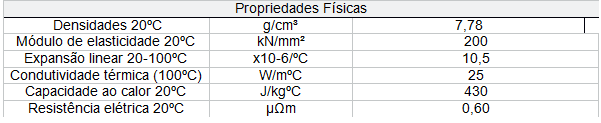
\includegraphics[scale = 1]{editaveis/figuras/propriedade_fisica_415}
    \label{prop_fisica415}
    \caption[Propriedades Físicas do Tp 415]{Propriedades Físicas do Tp 415}
   \end{figure}
   \FloatBarrier
   
    \begin{figure}[!h]
    \centering
    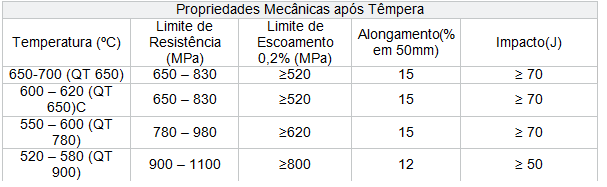
\includegraphics[scale = 1]{editaveis/figuras/propriedade_mecanica_tempera}
    \label{propriedade_tempera}
    \caption[Propriedades Mecânicas após Têmpera]{Propriedades Mecânicas após Têmpera}
   \end{figure}
   \FloatBarrier

Entramos em contato com alguns fornecedores que supostamente teriam este tipo de produto. A empresa chinesa Anhui Hummer Dynamo Co., Ltd, foi uma das destacadas por conter o produto em questão separadamente da turbina. Hummer é uma empresa de alta tecnologia especializada na indústria de energia eólica e está voltada para pesquisas, produção e serviço de médias-pequenas turbinas eólicas e atua em mais de 112 países, incluindo o Brasil.\footnotemark
\footnotetext{Disponível em:< http://www.chinahummer.cn >. Acesso em 20 Mai. 2015.}

O site Makepolo.com também foi visitado. Makepolo.com é um site fundada em 2007 que englobou cerca de 7000 sites de indústrias voltadas para a engenharia. A partir de 2012, mais de 1200 companhias do mundo a fora tem usado a plataforma para expor seus produtos e informações empresariais, dando a oportunidade para o cliente encontrar todas as informações em um só lugar.\footnotemark
 \footnotetext{Disponível em:< http://en.makepolo.com>. Acesso em 20 Mai. 2015.}
 
Enquanto não se obteve respostas dos fornecedores, a equipe decidiu estimar o preço levando em consideração o volume da torre e o preço da liga. Como temos as dimensões do raio inferior (R), raio superior (r), da altura (h) e da espessura da torre, estimou-se o volume (V) ocupado pelo aço por meio da expressão a seguir,  que indica o volume de um tronco de cone: \footnotemark
\footnotetext{Disponível em : < http://www.mundoeducacao.com/matematica/volume-tronco-cone.htm >. Acesso em 21 Mai. 2015.}
 \begin{figure}[!h]
    \centering
    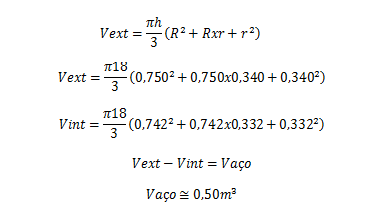
\includegraphics[scale = 1]{editaveis/figuras/equacao_torre}
    \label{eq_torre}
    \caption[Cálculo volume do tronco de cone externo]{Cálculo volume do tronco de cone externo}
   \end{figure}
   \FloatBarrier
  
Logo, calculamos o volume do tronco de cone externo e subtraímos deste o tronco de cone interno (com 8mm de espessura retirados do raio de cada diâmetro). Como temos a densidade do material (d=7,78 g/$cm^3$), calculamos a massa de aço estimada:
 \begin{figure}[!h]
    \centering
    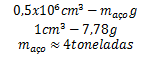
\includegraphics[scale = 1]{editaveis/figuras/massa_aco}
    \label{massa_aco}
    \caption[Cálculo da estimativa da massa do aço]{Cálculo da estimativa da massa do aço}
   \end{figure}
   \FloatBarrier
   
Com informações sobre o preço do aço Inox 415, fornecido pela companhia chinesa Henan Join-Win Im/Ex Corp, o preço da tonelada gira em torno de US\$750,00. \footnotemark Logo chegamos a uma quantia de US\$3.000,00 apenas de aço para a torre. Sabendo que em cima deste preço adiciona-se mão de obra, tratamentos térmicos, pinturas especializadas, testes entre outros fatores, este custo varia de acordo com a empresa que construísse a torre caso esta fosse projetada desde o início. Como se trata de uma estimativa de preço que espera-se da torre pronta pelo fornecedor, quintuplicamos a quantia de US\$3.000,00 e usamos o valor do dólar a R\$4,00, chegando a um valor estimado de R\$60.000,00 para cada torre de sustentação.
\footnotetext{Disponível em :< http://www.steel-jw.com.> Acesso em 22 Mai. 2015}

Levando em consideração as especificações da torre escolhida, a equipe propôs calcular a carga máxima que a torre é capaz de suportar levando em conta a flambagem, através da equação de Euler representada a seguir: 
 \begin{figure}[!h]
    \centering
    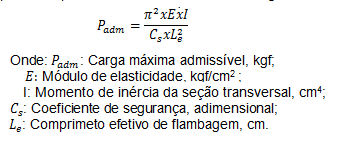
\includegraphics[scale = 1]{editaveis/figuras/eq_euler}
    \label{eq_euler}
    \caption[Equação de Euler]{Equação de Euler}
   \end{figure}
   \FloatBarrier
 
O momento de inércia depende das dimensões e formatos. Para o cálculo, utilizou-se o topo da torre como referência por ser o de menor valor, logo foi usado o momento de inércia para uma seção circular oca devido a presença de espessura na peça:
 \begin{figure}[!h]
    \centering
    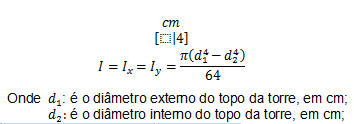
\includegraphics[scale = 1]{editaveis/figuras/mom_incercia}
    \label{mom_enercia}
    \caption[Equação do momento de inércia para uma seção circular oca]{Equação do momento de inércia para uma seção circular oca}
   \end{figure}
   \FloatBarrier
   
 O comprimento efetivo de flambagem foi usado considerando o caso de somente a base da torre está engastada, logo usa-se  $L_{e}=2L$, em cm \footnotemark. Tendo todos os valores, efetuando as devidas conversões utilizando ferramenta online \footnotemark substituindo as incógnitas nas expressões, temos: 
\footnotetext{Disponível em :< http://www.ufvjm.edu.br/disciplinas/agr006/files/2014/08/APOSTILA\_RESISTÊNCIAS\_DOS\_MATERIAIS.pdf i>. Acesso em 22 Mai. 2015}
\footnotetext{Disponível em:< http://www.translatorscafe.com/cafe/PT/units-converter/description/toc/>. Acesso em 22 Mai. 2015}
\begin{figure}[!h]
    \centering
    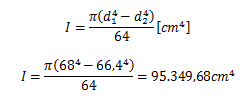
\includegraphics[scale = 1]{editaveis/figuras/calc_secao_circ}
    \label{calc_secao_circ}
    \caption[Cálculo do momento de inércia para uma seção circular oca]{Cálculo do momento de inércia para uma seção circular oca}
   \end{figure}
   \FloatBarrier
Utilizando um coeficiente de segurança de 3 para que previna deformações ou até mesmo o rompimento da estrutura e, convertendo o módulo de elasticidade de $200 kN/mm^2$ para $kgf/cm^2$, encontramos $2.039.432 kgf/cm^2$. Substituindo os valores na equação de Euler, tem-se:
\begin{figure}[!h]
    \centering
	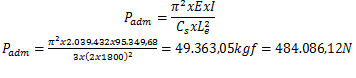
\includegraphics[scale = 1]{editaveis/figuras/calc_euler}
    \label{calc_euler}
    \caption[Cálculo da equação de Euler]{Cálculo da equação de Euler}
   \end{figure}
   \FloatBarrier
Sabendo que 1kgf equivale a 9,80665N, utilizando a fórmula da força gravítica (P = m x g) e supondo o valor da aceleração da gravidade $9,81 m/s^2$ \footnotemark, obtemos a massa máxima admissível pela torre de sustentação do presente projeto:
\footnotetext{Disponível em:< http://www.aulas-fisica-quimica.com/7f\_10.html>. Acesso em 23 Mai. 2015}
\begin{figure}[!h]
    \centering
	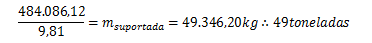
\includegraphics[scale = 1]{editaveis/figuras/massa_max}
    \label{massa_max}
    \caption[Massa máxima admissível pela torre de sustentação]{Massa máxima admissível pela torre de sustentação}
   \end{figure}
   \FloatBarrier
   
Pode-se concluir com este estudo realizado sobre a torre de sustentação, que uma carga de até 49 toneladas pode ser colocada no topo dessa peça sem que prejudique sua estabilidade, valor este que ultrapassa o valor estimado do peso de todos os componentes necessários para o funcionamento do sistema, assegurando assim a capacidade da torre de sustentação. O contato respondido confirmou o valor da estimativa feita, mesmo a torre sendo de um aço diferente, vemos uma relativa proximidade de preços. "The FOB Shanghai price of 18m freestanding tower for 50KW wind turbine is USD18.660,00 and the material is steel Q345".